
\documentclass[10pt]{article}

\def\Type{LessonDJ}
\def\TypeNum{Lesson 23}
\def\TypeTitle{Expected Value and Variance}
\def\Semester{Fall 2021} %Not Used 
\def\Course{MATH 1190 \& 1210}
\def\Targets{  {\bf\color{Orange}P3} }

\usepackage{preambleDJ}

%\usepackage{ragged2e}


%%%%%%%%%%%% BEGIN DOCUMENT %%%%%%%%%%%%%%%
%%%%%%%%%%%% BEGIN DOCUMENT %%%%%%%%%%%%%%%
%%%%%%%%%%%% BEGIN DOCUMENT %%%%%%%%%%%%%%%
%%%%%%%%%%%% BEGIN DOCUMENT %%%%%%%%%%%%%%%
%%%%%%%%%%%% BEGIN DOCUMENT %%%%%%%%%%%%%%%




\begin{document}

\pagestyle{otherpages}
\thispagestyle{firstpage}
\vs{.65}

In this lesson, we will explore two key measures used to describe the characteristics of random variables: the expectation (mean) and variance. Expectation measures the "average" or "expected" value of a random variable, while variance measures how much the values of the random variable deviates from this average.

\begin{center}
({\it Expectation, Variance \& Median of Discrete Random Variables})
\end{center}

\mpageT{.5}{.65}{
\fbox{$\mu=E[X] = \displaystyle\sum_{x\in S_X} x\cdot f(x)$} \vs{.1}~\\
  \fbox{$Var(X) = \displaystyle\sum_{x\in S_X} (x-\mu)^2\cdot f(x)$}
  }{\flushright
  \fbox{
\begin{minipage}{.7\textwidth}
The median, $m$, occurs when 
\enum{\item  $P(X\leq m) \geq 0.5$ {\em and} $P(X\geq m)\geq 0.5$.
\item If two values  (e.g $m_1$ and $m_2$) satisfy ($1$),}
 $$m=\dfrac{m_1+m_2}{2}$$
\end{minipage}
}
}

\exercise\ltrm{\bf\color{Orange}P3} In Lesson21 we  explored a fair coin whose sides are numbered ``$0$" and ``$1$" and flipped {\it three times}. We let $X$ represent the sum of the outcome of each flip, and found that the PMF of $X$ is given by
\mpageT{.5}{.5}{\large
\[ f(x)=\begin{cases}
\frac18 & \text{when }x=0\\
\frac38 & \text{when }x=1\\
\frac38 & \text{when }x=2\\
\frac18 & \text{when }x=3\\
0 & \text{otherwise}
\end{cases}\]
}{\centering
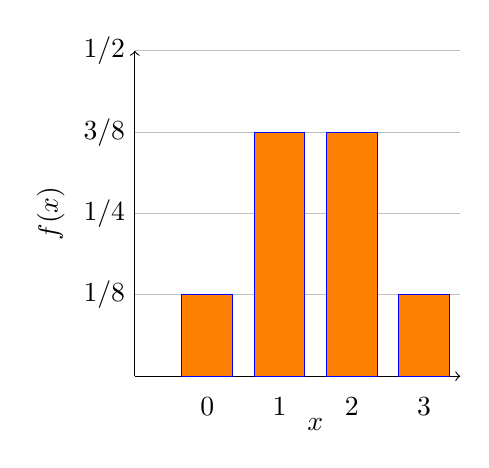
\begin{tikzpicture}
    \begin{axis}[
    y label style={anchor=south},
            ylabel={$f(x)$},
                        xlabel = {$x$},
	x label style={anchor=west},
        ybar, bar width=.7,
        ymajorgrids,
        axis lines*= left,
        width=\linewidth,
        xtick style= {draw=none}, ytick style= {draw=none},
   %t     enlargelimits=0.15,
        xtick={1,2,3,4},
        xticklabels={0,1,2,3},
        ytick={.125,.250,.375,.50},
        yticklabels={1/8,1/4,3/8,1/2},
         domain      = 0:4.5,
            restrict y to domain=0:0.5,
        xmin = 0, xmax = 4.5,
            ymin = 0, ymax = .5,
             axis line style={->},
             width = 2.25in, height=2.25in,
                 ]  
        \addplot[draw=blue, fill=orange] coordinates {(1,1/8) (2,3/8) (3,3/8) (4,1/8)};   
    \end{axis}
\end{tikzpicture}
}
\tasksA{2}{
\task  Before computing anything and basing your answer solely on the PMF above, how must the mean $\mu = E[X]$ and the median $m$ of $X$ be related?
\task Find $\mu=E[X]$.
\vs{1.5}
\task Find $Var(X)$.
}

%%%%%%%%%
\newpage%
%%%%%%%%%

\exercise\ltrm{\bf\color{Orange}P3} Each of the following histograms representing the PMFs of random variables $X_1$, $X_2$, and $X_3$ (respectively) were shown in pre-class activity. .
\mpageTth{.33}{.33}{.33}{
  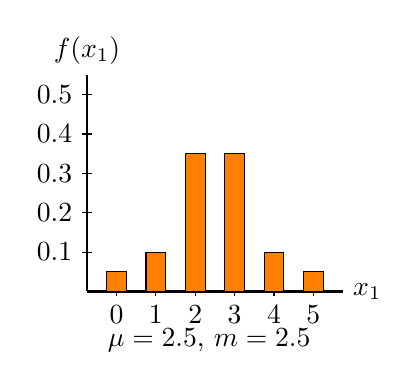
\begin{tikzpicture}
    [scale=0.25]
    %axes
    \draw[thick](0,0)--(0,11) node[above]{$f(x_1)$};
    \draw[thick](0,0)--(13,0) node[right]{$x_1$};
    %label horizontal axis
    \draw (1.5,0.25)--(1.5,-0.25) node[below]{$0$};
    \draw (3.5,0.25)--(3.5,-0.25) node[below]{$1$};
    \draw (5.5,0.25)--(5.5,-0.25) node[below]{$2$};
    \draw (7.5,0.25)--(7.5,-0.25) node[below]{$3$};
    \draw (9.5,0.25)--(9.5,-0.25)
    node[below]{$4$};
    \draw (11.5,0.25)--(11.5,-0.25)
    node[below]{$5$};
    %label vertical axis
    \draw (0.25,2)--(-0.25,2) node[left]{$0.1$};
    \draw (0.25,4)--(-0.25,4) node[left]{$0.2$};
    \draw (0.25,6)--(-0.25,6) node[left]{$0.3$};
    \draw (0.25,8)--(-0.25,8) node[left]{$0.4$};
    \draw (0.25,10)--(-0.25,10) node[left]{$0.5$};
    %histogram
    \draw[fill=orange] (1,0)--(2,0)--(2,1)--(1,1)--(1,0);
    \draw[fill=orange] (3,0)--(3,2)--(4,2)--(4,0)--(3,0);
    \draw[fill=orange] (5,0)--(5,7)--(6,7)--(6,0)--(5,0);
    \draw[fill=orange] (7,0)--(8,0)--(8,7)--(7,7)--(7,0);
    \draw[fill=orange] (9,0)--(10,0)--(10,2)--(9,2)--(9,0);
    \draw[fill=orange]
    (11,0)--(12,0)--(12,1)--(11,1)--(11,0);
    \node[below=1em] at (current bounding box.base) {$\mu=2.5$, $m=2.5$};
    \end{tikzpicture}
}{
 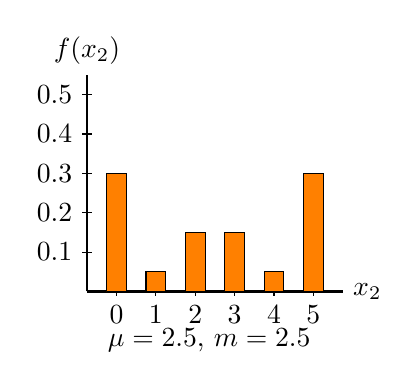
\begin{tikzpicture}
    [scale=0.25]
    %axes
    \draw[thick](0,0)--(0,11) node[above]{$f(x_2)$};
    \draw[thick](0,0)--(13,0) node[right]{$x_2$};
    %label horizontal axis
    \draw (1.5,0.25)--(1.5,-0.25) node[below]{$0$};
    \draw (3.5,0.25)--(3.5,-0.25) node[below]{$1$};
    \draw (5.5,0.25)--(5.5,-0.25) node[below]{$2$};
    \draw (7.5,0.25)--(7.5,-0.25) node[below]{$3$};
    \draw (9.5,0.25)--(9.5,-0.25)
    node[below]{$4$};
    \draw (11.5,0.25)--(11.5,-0.25)
    node[below]{$5$};
    %label vertical axis
    \draw (0.25,2)--(-0.25,2) node[left]{$0.1$};
    \draw (0.25,4)--(-0.25,4) node[left]{$0.2$};
    \draw (0.25,6)--(-0.25,6) node[left]{$0.3$};
    \draw (0.25,8)--(-0.25,8) node[left]{$0.4$};
    \draw (0.25,10)--(-0.25,10) node[left]{$0.5$};
    %histogram
    \draw[fill=orange] (1,0)--(2,0)--(2,6)--(1,6)--(1,0);
    \draw[fill=orange] (3,0)--(3,1)--(4,1)--(4,0)--(3,0);
    \draw[fill=orange] (5,0)--(5,3)--(6,3)--(6,0)--(5,0);
    \draw[fill=orange] (7,0)--(8,0)--(8,3)--(7,3)--(7,0);
    \draw[fill=orange] (9,0)--(10,0)--(10,1)--(9,1)--(9,0);
    \draw[fill=orange]
    (11,0)--(12,0)--(12,6)--(11,6)--(11,0);
        \node[below=1em] at (current bounding box.base) {$\mu=2.5$, $m=2.5$};
    \end{tikzpicture}
}{
    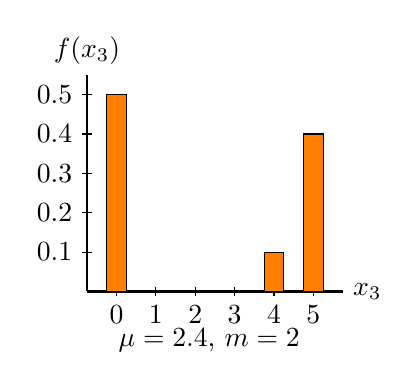
\begin{tikzpicture}
    [scale=0.25]
    %axes
    \draw[thick](0,0)--(0,11) node[above]{$f(x_3)$};
    \draw[thick](0,0)--(13,0) node[right]{$x_3$};
    %label horizontal axis
    \draw (1.5,0.25)--(1.5,-0.25) node[below]{$0$};
    \draw (3.5,0.25)--(3.5,-0.25) node[below]{$1$};
    \draw (5.5,0.25)--(5.5,-0.25) node[below]{$2$};
    \draw (7.5,0.25)--(7.5,-0.25) node[below]{$3$};
    \draw (9.5,0.25)--(9.5,-0.25)
    node[below]{$4$};
    \draw (11.5,0.25)--(11.5,-0.25)
    node[below]{$5$};
    %label vertical axis
    \draw (0.25,2)--(-0.25,2) node[left]{$0.1$};
    \draw (0.25,4)--(-0.25,4) node[left]{$0.2$};
    \draw (0.25,6)--(-0.25,6) node[left]{$0.3$};
    \draw (0.25,8)--(-0.25,8) node[left]{$0.4$};
    \draw (0.25,10)--(-0.25,10) node[left]{$0.5$};
    %histogram
    \draw[fill=orange] (1,0)--(2,0)--(2,10)--(1,10)--(1,0);
    \draw[fill=orange] (3,0)--(3,0)--(4,0)--(4,0)--(3,0);
    \draw[fill=orange] (5,0)--(5,0)--(6,0)--(6,0)--(5,0);
    \draw[fill=orange] (7,0)--(8,0)--(8,0)--(7,0)--(7,0);
    \draw[fill=orange] (9,0)--(10,0)--(10,2)--(9,2)--(9,0);
    \draw[fill=orange]
    (11,0)--(12,0)--(12,8)--(11,8)--(11,0);
            \node[below=1em] at (current bounding box.base) {$\mu=2.4$, $m=2$};
    \end{tikzpicture}
    }
    
\enumA{
\item Before computing anything and basing your answer solely on the PMF above, put the variances of the three random variables in order from least to greatest. Consider how variance is related to the mean, $\mu$ in each of the three examples.  Explain your reasoning. \vs{1.5}\\
\mpageT{.5}{.5}[\hs{.2}]{
\item Sketch an example of a histogram representing the PMF of a random variable $Y$ having {\bf higher} variance than $X_3$. \\
\begin{center}
\begin{tikzpicture}
    [scale=0.35]
    %axes
    \draw[thick](0,0)--(0,11) node[above]{$f(y)$};
    \draw[thick](0,0)--(13,0) node[right]{$y$};
    %label horizontal axis
    \draw (1.5,0.25)--(1.5,-0.25) node[below]{$0$};
    \draw (3.5,0.25)--(3.5,-0.25) node[below]{$1$};
    \draw (5.5,0.25)--(5.5,-0.25) node[below]{$2$};
    \draw (7.5,0.25)--(7.5,-0.25) node[below]{$3$};
    \draw (9.5,0.25)--(9.5,-0.25)
    node[below]{$4$};
    \draw (11.5,0.25)--(11.5,-0.25)
    node[below]{$5$};
    %label vertical axis
    \draw (0.25,2)--(-0.25,2) node[left]{$0.1$};
    \draw (0.25,4)--(-0.25,4) node[left]{$0.2$};
    \draw (0.25,6)--(-0.25,6) node[left]{$0.3$};
    \draw (0.25,8)--(-0.25,8) node[left]{$0.4$};
    \draw (0.25,10)--(-0.25,10) node[left]{$0.5$};
    %histogram
    %\draw[fill=orange] (1,0)--(2,0)--(2,10)--(1,10)--(1,0);
    %\draw[fill=orange] (3,0)--(3,0)--(4,0)--(4,0)--(3,0);
    %\draw[fill=orange] (5,0)--(5,0)--(6,0)--(6,0)--(5,0);
    %\draw[fill=orange] (7,0)--(8,0)--(8,0)--(7,0)--(7,0);
    %\draw[fill=orange] (9,0)--(10,0)--(10,2)--(9,2)--(9,0);
    %\draw[fill=orange]
    (11,0)--(12,0)--(12,8)--(11,8)--(11,0);
\end{tikzpicture}
\end{center}
}{
\item Sketch an example of a histogram representing the PMF of a random variable $Z$ having the same mean as $X_1$ but {\bf lower} variance than $X_1$.\\
\begin{center}
\begin{tikzpicture}
    [scale=0.35]
    %axes
    \draw[thick](0,0)--(0,11) node[above]{$f(z)$};
    \draw[thick](0,0)--(13,0) node[right]{$z$};
    %label horizontal axis
    \draw (1.5,0.25)--(1.5,-0.25) node[below]{$0$};
    \draw (3.5,0.25)--(3.5,-0.25) node[below]{$1$};
    \draw (5.5,0.25)--(5.5,-0.25) node[below]{$2$};
    \draw (7.5,0.25)--(7.5,-0.25) node[below]{$3$};
    \draw (9.5,0.25)--(9.5,-0.25)
    node[below]{$4$};
    \draw (11.5,0.25)--(11.5,-0.25)
    node[below]{$5$};
    %label vertical axis
    \draw (0.25,2)--(-0.25,2) node[left]{$0.1$};
    \draw (0.25,4)--(-0.25,4) node[left]{$0.2$};
    \draw (0.25,6)--(-0.25,6) node[left]{$0.3$};
    \draw (0.25,8)--(-0.25,8) node[left]{$0.4$};
    \draw (0.25,10)--(-0.25,10) node[left]{$0.5$};
    %histogram
    %\draw[fill=orange] (1,0)--(2,0)--(2,10)--(1,10)--(1,0);
    %\draw[fill=orange] (3,0)--(3,0)--(4,0)--(4,0)--(3,0);
    %\draw[fill=orange] (5,0)--(5,0)--(6,0)--(6,0)--(5,0);
    %\draw[fill=orange] (7,0)--(8,0)--(8,0)--(7,0)--(7,0);
    %\draw[fill=orange] (9,0)--(10,0)--(10,2)--(9,2)--(9,0);
    %\draw[fill=orange]
    (11,0)--(12,0)--(12,8)--(11,8)--(11,0);
\end{tikzpicture}
\end{center}
}
}

\begin{center}
({\bf Note:} don't forget that the total probability must be exactly 1.)
\end{center}

\newpage

\begin{center}
({\it Expectation, Variance \& Median of Continuous Random Variables})
\end{center}
\mpageT{.5}{.5}{
\centering
\fbox{$\mu=E[X] = \displaystyle\int_{S_X} x\cdot f(x)\,dx$} \vs{.1}~\\
\fbox{$Var(X) = \displaystyle\int_{S_X} (x-\mu)^2\cdot f(x)\,dx$}
  }{
  \fbox{
\begin{minipage}{.8\textwidth}
The median, $m$, occurs when
 $$P(X\leq m) = 0.5 \Rightarrow \int_{-\infty}^m f(x)\;dx=0.5$$
\end{minipage}
}
}


%\,\hfill \fbox{$\mu=E[X] = \displaystyle\int_{S_X} x\cdot f(x)\,dx$} \hfill \fbox{$Var(X) = \displaystyle\int_{S_X} (x-\mu)^2\cdot f(x)\,dx$} \hfill\,

\exercise\ltrm{{\bf\color{Orange}P3}} Let the continuous random variable $V$ have the following PDF:
\[
f(v) = 
\begin{cases} 
\frac{1}{v} & \text{for } 1 \leq v \leq e, \\
0 & \text{otherwise}.
\end{cases}
\]

\begin{itemize}
\item[(a)] Find the mean of $V$, $\mu=E(V)$.
   \vs{2}


\item[(b)] Find the variance of $V$, $Var(V)$.
\end{itemize}
\newpage



\exercise\ltrm{{\bf\color{Orange}P3}} The integral $\dint_1^{?} \frac12z\,dz$ represents the expected value of a random variable $Z$.\\

\tasksA{2}{
\task  Find the PDF, $f(z)$.  \\
{\em Hint 1}: Focus on the definition of $E(X)$ above.  {\em Hint 2}: Ignore the $?$ in the upper bound of the integral for now.
\task  Find the support of $Z$. \\{\em Hint}: Find the value of $?$ to ensure $f(z)$ is a PDF.  
 \vs{4}
\task Find the mean of $Z$.
\task Find the variance of $Z$.
}


%%%%%%%%%
\newpage%
%%%%%%%%%

{\bf\color{blue}Extra Practice 1.} \ltrm{{\bf\color{Orange}P3}}
Consider a random variable \(X\) that takes integer values from 1 to 5 with frequencies as shown in the histogram below:

\begin{center}
\begin{minipage}[t]{0.45\textwidth}
\,\\[-0.2in]
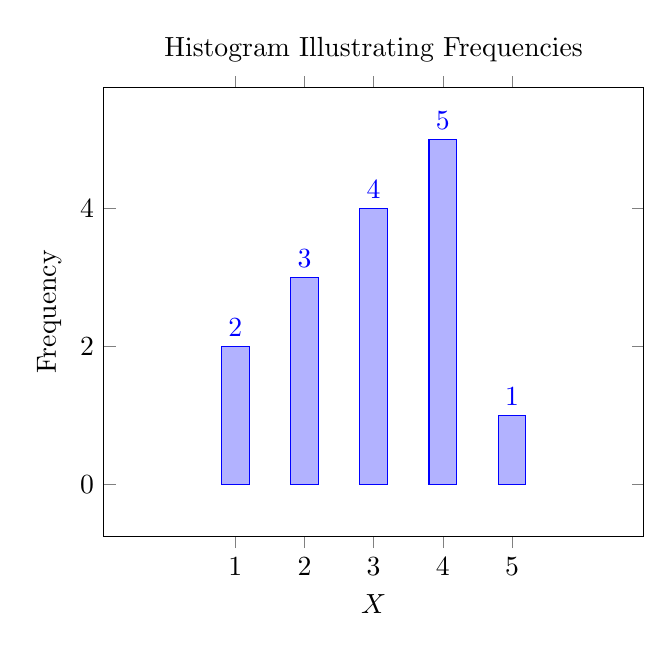
\begin{tikzpicture}
  \begin{axis}[
      ybar,
      xlabel={\(X\)},
      ylabel={Frequency},
      ymin=0,
      xmin=0, xmax=6,
      bar width=0.4,
      xtick={1,2,3,4,5},
      nodes near coords,
      enlargelimits=0.15,
      title={Histogram Illustrating Frequencies}
  ]
  \addplot coordinates {(1,2) (2,3) (3,4) (4,5) (5,1)};
  \end{axis}
\end{tikzpicture}
\end{minipage}
%
\quad
%
\begin{minipage}[t]{0.45\textwidth}
\vspace{0.5in}
\begin{itemize}
    \item \(X = 1\) has a frequency of 2.
    \item \(X = 2\) has a frequency of 3.
    \item \(X = 3\) has a frequency of 4.
    \item \(X = 4\) has a frequency of 5.
    \item \(X = 5\) has a frequency of 1.
\end{itemize}
\end{minipage}
\end{center}


\begin{itemize}
\item[(a)] Based solely on the histogram above, how are the mean and median of $X$ related? Explain.
    \vfill

\item[(b)] Calculate the expected value (mean) of the random variable \(X\). ({\bf Note:} frequencies are given in the histogram above - not probabilities.)
    \vfill

\item[(c)] Calculate the median of the random variable $X$. ({\bf Note:} frequencies are given in the histogram above - not probabilities.)
    \vfill
    
\end{itemize}

%%%%%%%%%
\newpage%
%%%%%%%%%

{\bf\color{blue}Extra Practice 2.}\ltrm{{\bf\color{Orange}P3}}
Compute the expectation of a continuous random variable $W$ with PDF given by:
\[
f(w) = 
\begin{cases} 
2\sqrt{w} & \text{for } 0 \leq w \leq 1, \\
0 & \text{otherwise}.
\end{cases}
\]

\vfill

{\bf\color{blue}Extra Practice 3.}\ltrm{{\bf\color{Orange}P3}} 
Let $X$ be a continuous random variable with the following PDF:
\[
f(x) = \frac{1}{x \ln(10)} \quad \text{for } 1 \leq x \leq 10, \quad \text{and } 0 \text{ otherwise}.
\]
\begin{itemize}
    \item[(a)] Compute the expectation $\mu=E[X]$.
        \vfill
    \item[(b)] Determine the variance $\text{Var}(X)$. You may leave your answer in terms of $\mu$.
        \vfill
        \vfill
\end{itemize}

\end{document}